%Version 2.1 April 2023
% See section 11 of the User Manual for version history
%
%%%%%%%%%%%%%%%%%%%%%%%%%%%%%%%%%%%%%%%%%%%%%%%%%%%%%%%%%%%%%%%%%%%%%%
%%                                                                 %%
%% Please do not use \input{...} to include other tex files.       %%
%% Submit your LaTeX manuscript as one .tex document.              %%
%%                                                                 %%
%% All additional figures and files should be attached             %%
%% separately and not embedded in the \TeX\ document itself.       %%
%%                                                                 %%
%%%%%%%%%%%%%%%%%%%%%%%%%%%%%%%%%%%%%%%%%%%%%%%%%%%%%%%%%%%%%%%%%%%%%

%%\documentclass[referee,sn-basic]{sn-jnl}% referee option is meant for double line spacing

%%=======================================================%%
%% to print line numbers in the margin use lineno option %%
%%=======================================================%%

%%\documentclass[lineno,sn-basic]{sn-jnl}% Basic Springer Nature Reference Style/Chemistry Reference Style

%%======================================================%%
%% to compile with pdflatex/xelatex use pdflatex option %%
%%======================================================%%

%%\documentclass[pdflatex,sn-basic]{sn-jnl}% Basic Springer Nature Reference Style/Chemistry Reference Style


%%Note: the following reference styles support Namedate and Numbered referencing. By default the style follows the most common style. To switch between the options you can add or remove �Numbered� in the optional parenthesis. 
%%The option is available for: sn-basic.bst, sn-vancouver.bst, sn-chicago.bst, sn-mathphys.bst. %  
 
%%\documentclass[sn-nature]{sn-jnl}% Style for submissions to Nature Portfolio journals
%%\documentclass[sn-basic]{sn-jnl}% Basic Springer Nature Reference Style/Chemistry Reference Style
\documentclass[sn-mathphys,Numbered]{sn-jnl}% Math and Physical Sciences Reference Style
%%\documentclass[sn-aps]{sn-jnl}% American Physical Society (APS) Reference Style
%%\documentclass[sn-vancouver,Numbered]{sn-jnl}% Vancouver Reference Style
%%\documentclass[sn-apa]{sn-jnl}% APA Reference Style 
%%\documentclass[sn-chicago]{sn-jnl}% Chicago-based Humanities Reference Style
%%\documentclass[default]{sn-jnl}% Default
%%\documentclass[default,iicol]{sn-jnl}% Default with double column layout

%%%% Standard Packages
%%<additional latex packages if required can be included here>

\usepackage{graphicx}%
\usepackage{multirow}%
\usepackage{amsmath,amssymb,amsfonts}%
\usepackage{amsthm}%
\usepackage{mathrsfs}%
\usepackage[title]{appendix}%
\usepackage{xcolor}%
\usepackage{textcomp}%
\usepackage{manyfoot}%
\usepackage{booktabs}%
\usepackage{algorithm}%
\usepackage{algorithmicx}%
\usepackage{algpseudocode}%
\usepackage{listings}%
%%%%

%%%%%=============================================================================%%%%
%%%%  Remarks: This template is provided to aid authors with the preparation
%%%%  of original research articles intended for submission to journals published 
%%%%  by Springer Nature. The guidance has been prepared in partnership with 
%%%%  production teams to conform to Springer Nature technical requirements. 
%%%%  Editorial and presentation requirements differ among journal portfolios and 
%%%%  research disciplines. You may find sections in this template are irrelevant 
%%%%  to your work and are empowered to omit any such section if allowed by the 
%%%%  journal you intend to submit to. The submission guidelines and policies 
%%%%  of the journal take precedence. A detailed User Manual is available in the 
%%%%  template package for technical guidance.
%%%%%=============================================================================%%%%

%\jyear{2021}%

%% as per the requirement new theorem styles can be included as shown below
\theoremstyle{thmstyleone}%
\newtheorem{theorem}{Theorem}%  meant for continuous numbers
%%\newtheorem{theorem}{Theorem}[section]% meant for sectionwise numbers
%% optional argument [theorem] produces theorem numbering sequence instead of independent numbers for Proposition
\newtheorem{proposition}[theorem]{Proposition}% 
%%\newtheorem{proposition}{Proposition}% to get separate numbers for theorem and proposition etc.

\theoremstyle{thmstyletwo}%
\newtheorem{example}{Example}%
\newtheorem{remark}{Remark}%

\theoremstyle{thmstylethree}%
\newtheorem{definition}{Definition}%

\raggedbottom
%%\unnumbered% uncomment this for unnumbered level heads

\begin{document}

\title[Article Title]{Article Title}

%%=============================================================%%
%% Prefix	-> \pfx{Dr}
%% GivenName	-> \fnm{Joergen W.}
%% Particle	-> \spfx{van der} -> surname prefix
%% FamilyName	-> \sur{Ploeg}
%% Suffix	-> \sfx{IV}
%% NatureName	-> \tanm{Poet Laureate} -> Title after name
%% Degrees	-> \dgr{MSc, PhD}
%% \author*[1,2]{\pfx{Dr} \fnm{Joergen W.} \spfx{van der} \sur{Ploeg} \sfx{IV} \tanm{Poet Laureate} 
%%                 \dgr{MSc, PhD}}\email{iauthor@gmail.com}
%%=============================================================%%

\author*[1,2]{\fnm{First} \sur{Author}}\email{iauthor@gmail.com}

\author[2,3]{\fnm{Second} \sur{Author}}\email{iiauthor@gmail.com}
\equalcont{These authors contributed equally to this work.}

\author[1,2]{\fnm{Third} \sur{Author}}\email{iiiauthor@gmail.com}
\equalcont{These authors contributed equally to this work.}

\affil*[1]{\orgdiv{Department}, \orgname{Organization}, \orgaddress{\street{Street}, \city{City}, \postcode{100190}, \state{State}, \country{Country}}}

\affil[2]{\orgdiv{Department}, \orgname{Organization}, \orgaddress{\street{Street}, \city{City}, \postcode{10587}, \state{State}, \country{Country}}}

\affil[3]{\orgdiv{Department}, \orgname{Organization}, \orgaddress{\street{Street}, \city{City}, \postcode{610101}, \state{State}, \country{Country}}}

%%==================================%%
%% sample for unstructured abstract %%
%%==================================%%

\abstract{The abstract serves both as a general introduction to the topic and as a brief, non-technical summary of the main results and their implications. Authors are advised to check the author instructions for the journal they are submitting to for word limits and if structural elements like subheadings, citations, or equations are permitted.}

%%================================%%
%% Sample for structured abstract %%
%%================================%%

% \abstract{\textbf{Purpose:} The abstract serves both as a general introduction to the topic and as a brief, non-technical summary of the main results and their implications. The abstract must not include subheadings (unless expressly permitted in the journal's Instructions to Authors), equations or citations. As a guide the abstract should not exceed 200 words. Most journals do not set a hard limit however authors are advised to check the author instructions for the journal they are submitting to.
% 
% \textbf{Methods:} The abstract serves both as a general introduction to the topic and as a brief, non-technical summary of the main results and their implications. The abstract must not include subheadings (unless expressly permitted in the journal's Instructions to Authors), equations or citations. As a guide the abstract should not exceed 200 words. Most journals do not set a hard limit however authors are advised to check the author instructions for the journal they are submitting to.
% 
% \textbf{Results:} The abstract serves both as a general introduction to the topic and as a brief, non-technical summary of the main results and their implications. The abstract must not include subheadings (unless expressly permitted in the journal's Instructions to Authors), equations or citations. As a guide the abstract should not exceed 200 words. Most journals do not set a hard limit however authors are advised to check the author instructions for the journal they are submitting to.
% 
% \textbf{Conclusion:} The abstract serves both as a general introduction to the topic and as a brief, non-technical summary of the main results and their implications. The abstract must not include subheadings (unless expressly permitted in the journal's Instructions to Authors), equations or citations. As a guide the abstract should not exceed 200 words. Most journals do not set a hard limit however authors are advised to check the author instructions for the journal they are submitting to.}

\keywords{keyword1, Keyword2, Keyword3, Keyword4}

%%\pacs[JEL Classification]{D8, H51}

%%\pacs[MSC Classification]{35A01, 65L10, 65L12, 65L20, 65L70}

\maketitle

\section{Introduction}
Improving the efficiency of working fluids in thermo systems enhances their overall performance and minimizes size requirements. Nanofluids, which are suspensions of small percentages (<5 vol.  \%) of various nanoparticles in conventional working fluids, have emerged as an excellent solution to address the thermal challenges in advanced heat transfer systems.

In a study by Pak and Cho on nanofluids consisting of 3 vol.  \% 27 nm titanium dioxide particles in water, a new correlation for turbulent convective heat transfer in dilute nanofluids was reported \cite{ref1}:

\begin{equation}
	\mathbf{Nu} = 0.21 \mathbf{Re}^{0.8} \mathbf{Pr}^{0.5}
\end{equation}

where  \textbf{Nu} is the Nusselt number,  \textbf{Re}  is the Reynolds number, and  \textbf{Pr} is the Prandtl number and $ 6.54 \leq \text{Pr} \leq 12.33, \quad \begin{matrix}
	10^4 \leq \text{Re} \leq 10^5
\end{matrix} $

He et al. synthesized stable aqueous 20 nm titanium dioxide nanofluids with different agglomerate sizes and concentrations, revealing an increase in convective heat transfer coefficient with nanoparticle concentration, particularly in turbulent flow regimes \cite{ref2}.


\section{Related Works}

While experimental studies provide valuable insights, more research is needed to model the intricate processes and establish empirical relations between effective parameters. Artificial neural networks (ANNs) have proven effective in modeling various processes. For instance, Santra et al. applied ANN to predict heat transfer in laminar natural convection of copper?water nanofluids, demonstrating accurate predictions within the training data range \cite{ref3}. Fazeli et al. utilized ANN to simulate the heat transfer characteristics of a miniature heat sink cooled by SiO2?water nanofluids, achieving excellent agreement with mathematical simulations \cite{ref4}. Balcilar et al. employed ANNs to determine parameters' effects on the heat transfer coefficient of nanofluids, showing good agreement with experimental data \cite{ref5}.

Papari et al. utilized ANN analysis to estimate the thermal conductivity of nanofluids containing multi-walled carbon nanotubes (MWCNTs) and single-walled carbon nanotubes (SWCNTs), with predicted values in good agreement with literature \cite{ref6}. Hojjat et al. synthesized various nanofluids and proposed neural network models to represent thermal conductivity as a function of temperature, nanoparticle concentration, and the thermal conductivity of nanoparticles \cite{ref7}.

In this paper, we employ neural networks to estimate the forced convective heat transfer coefficient of nanofluids. The study aims to compare the modeling results with experimental data obtained for water and an ethylene glycol/water mixture as the base fluid. Nanofluids containing TiO2 nanoparticles at various concentrations will be tested under different heat flux boundary conditions, flowing upward through a vertical pipe in laminar and turbulent flow regimes.


\section{Experimental Setup}
Spherical titanium dioxide nanoparticles dispersed in distilled water and ethylene glycol/water mixture (60 weight-\% ethylene glycol) were used. Nanoparticles were purchased from Degussa (Germany) with an average diameter of 25 nm. An ultrasonic vibrator (Tecna 6) was used for the preparation of mixed aqueous suspensions. The suspension was sonicated for 4 hours at a frequency of 50-60 kHz with an output power of 138W, at 65 C, and pH=11 by NaOH solution. Nanofluids containing 0.5\%, 1.0\%, 1.5\% titanium dioxide by volume were obtained using the two-step method. The stability time of nanofluids was observed to be 24 hours without any stabilizer.

The test section in Fig. 1 (experimental apparatus) was a straight copper tube with a length of 120 cm, an inner diameter of 6 mm, and an outer diameter of 8 mm. Two rods of heaters with different AC power in parallel with the tube were used as heaters with a thick thermal isolating layer. Four (K-type) thermocouples were welded on the inner tube wall at 20 cm (Tw1), 50 cm (Tw2), 80 cm (Tw3), and 110 cm (Tw4) from the inlet of the test section. Two further K-type thermocouples were inserted into the flow at 8 cm (Tfin) and 119 cm (Tfout) from the inlet of the test section. After injection of nanofluid into a glass vessel as a fluid reservoir tank, it was circulated toward the test section using a pump (STAR RS 25/6-130). Flow rate was measured by a flow meter, and different flow rates (0.5-5.0 L/min) were obtained by using a valve before the flow meter. To cool nanofluids, a tube-in-shell type heat exchanger was used.


% Paste this into your TexStudio document

\subsection{Problem Formulation}
The experimental data served as the basis for calculating the convective heat transfer coefficient ($h$) and Nusselt number ($Nu$) using the following equations:

\begin{equation}
	q = h \cdot (T_{3i} - T_f) \quad \text{(2)}
\end{equation}

where $q$ is the heat flux, $T_w$ is the measured wall temperature, and $T_f$ is the fluid temperature calculated through the energy balance equation:

\begin{equation}
	q = \rho_f \cdot c_f \cdot Q \cdot (T_{\text{fin}} - T_f) \quad \text{(3)}
\end{equation}

Here, $T_{\text{fin}}$ is the measured fluid temperature at the inlet of the test section, $c_f$ is the fluid heat capacity, $\rho_f$ is the fluid density, $S$ is the perimeter of the test tube, and $Q$ is the flow rate. For nanofluids, the value of $\rho c$ was calculated using the equation:

\begin{equation}
	\rho c = \rho_f \cdot c_f + \rho_p \cdot c_p \cdot VF \quad \text{(4)}
\end{equation}

Comparing the measured fluid temperature at the outlet of the test section with the theoretical value calculated by Eq. (3) revealed a maximum deviation lower than 12% under the conditions of this study.

The convective heat transfer coefficient, $h$, in Eq. (2), is often expressed in the form of the Nusselt number ($Nu$):

\begin{equation}
	Nu = \frac{h \cdot D}{k_f} \quad \text{(5)}
\end{equation}

Here, $D$ is the tube inner diameter, and $k_f$ is the fluid thermal conductivity. For nanofluids, $k_f$ is predicted by the H-C model \cite{ref8}:

\begin{equation}
	k_f = k_f \cdot [1 + 2.5 \cdot \phi] \quad \text{(6)}
\end{equation}

where $\phi$ is the volume fraction of nanoparticles. Additionally, the Nusselt number is traditionally related to the Reynolds number ($Re$) and the Prandtl number ($Pr$):

\begin{equation}
	Nu = C \cdot Re^m \cdot Pr^n \quad \text{(7)}
\end{equation}

where $C$, $m$, and $n$ are constants. The Reynolds number ($Re$) and the Prandtl number ($Pr$) are defined as:

\begin{equation}
	Re = \frac{\rho_f \cdot u \cdot D}{\mu_f} \quad \text{(8)}
\end{equation}

\begin{equation}
	Pr = \frac{\mu_f \cdot c_f}{k_f} \quad \text{(9)}
\end{equation}

For nanofluids, the Prandtl number is predicted by the Einstein equation. In Eq. (7), $x$ represents the axial distance from the entrance of the test section.



\section{Modeling}

In this study, an artificial neural network (ANN) program was developed using the MATLAB software environment. A total of 56 experimental datasets, derived from various experiments, were utilized to construct a three-layer feed-forward neural network model. The hyperbolic tangent sigmoid (\texttt{tansig}) transfer function with a back-propagation algorithm at the hidden layer and a linear transfer function (\texttt{purelin}) at the output layer were employed.

To enhance the numerical stability (accuracy index) of the model construction, both inputs and targets were initially normalized to produce data with zero mean and unity standard deviation. Principal component analysis (PCA) was then performed before the training stage. The number of principal components, accounting for 98\% of the variation, equaled the number of original input parameters, indicating no redundancy in the dataset.

Next, the datasets were divided into three sets: a training dataset comprising one-half of the data for training the ANN, a validation dataset with one-quarter of the data for validating the developed ANN, and a testing set with one-quarter of the data for evaluating the ANN. Various learning algorithms were applied to select the best one, followed by optimization between the neuron number and mean squared error (MSE) for the chosen learning algorithm.

Different statistical parameters, such as mean absolute error (MAE), MSE, root mean squared error (RMSE), and determination coefficient ($R^2$), were calculated to assess the accuracy of the modeling process.



\section{Results and Discussion}

\subsection{Learning Algorithm Selection}

To identify the optimal back-propagation learning algorithm, various algorithms were employed. A three-layer feed-forward artificial neural network (ANN) with a hyperbolic tangent sigmoid (\texttt{tansig}) transfer function at the hidden layer and a linear (\texttt{purelin}) transfer function at the output layer was utilized for all back-propagation learning algorithms. Ten neurons were consistently used in the hidden layer for all algorithms. The results are summarized in Table 1.

\begin{table}[ht]
	\centering
	\begin{tabular}{|c|c|}
		\hline
		\textbf{Learning Algorithm} & \textbf{Minimum MSE} \\ \hline
		Levenberg?Marquardt (LM)   & 0.0010              \\ \hline
	\end{tabular}
	\caption{Performance comparison of back-propagation learning algorithms.}
	\label{tab:learning_algorithms}
\end{table}

As evident from Table 1, the Levenberg?Marquardt (LM) algorithm exhibited the lowest Mean Squared Error (MSE) of 0.0010, establishing it as the most effective back-propagation learning algorithm.

\subsection{Optimization of Artificial Neural Network}

The number of hidden layer neurons significantly influences the performance of artificial neural networks (ANNs). Inappropriately low values hinder proper training, while excessively high values lead to overfitting \cite{ref11}. The optimal number of neurons in the hidden layer was determined through trial and error, ranging from 2 to 9 neurons. The relationship between the number of hidden layer neurons and MSE is presented in Table 2. The minimum MSE value of 0.0008 was observed with 6 neurons in the hidden layer. Consequently, the ANN was configured with 6 neurons in the hidden layer.

\begin{table}10ht]
	\centering
	\begin{tabular}{|c|c|}
		\hline
		\textbf{Number of Neurons in Hidden Layer} & \textbf{MSE} \\ \hline
		2                                          & 0.0021      \\ \hline
		4                                          & 0.0015      \\ \hline
		6                                          & 0.0008      \\ \hline
		8                                          & 0.0013      \\ \hline
		9                                          & 0.0016      \\ \hline
	\end{tabular}
	\caption{Optimization of the number of neurons in the hidden layer.}
	\label{tab:hidden_layer_neurons}
\end{table}

\subsection{Convective Heat Transfer Coefficient of Distilled Water}

The experimental system was tested with distilled water at Reynolds numbers of 2960 and 3960. To validate the constant heat flux boundary condition, the experimental data of the convective heat transfer coefficient of distilled water, represented as the Nusselt number (Nu), was compared with the predicted Nu number from the Gnielinski equation \cite{ref9}. The Gnielinski equation for constant heat flux boundary conditions is given by:

\begin{equation}
	Nu = \left(0.155 \cdot Re^{0.33}\right) \cdot Pr^{0.33}
	\label{eq:gniellinski}
\end{equation}

The experimental and predicted Nu numbers for Reynolds numbers 2960 and 3960 are shown in Figures 2(a) and 2(b). The Gnielinski equation predicts the experimental data with a 4 \% deviation for $Re = 2960$ and a 3 \% deviation for $Re = 3960$. These deviations are attributed to the influence of the entrance on the heat transfer coefficient, not accounted for in Eq.~(\ref{eq:gniellinski}). Therefore, the constant heat flux boundary condition for this study is deemed valid.

\subsection{Effect of Nanoparticle Concentrations on the Convective Heat Transfer Coefficient in Distilled Water}

In Figures 3(a) and 3(b), the experimental results and predicted data from the ANN were compared. The axial profiles of the heat transfer coefficient of nanofluids show an increase with increasing particle concentration. The enhancement is more pronounced at higher Reynolds numbers. For instance, at $Re = 2960$ and $Re = 3960$, the maximum enhancement with 1.50 vol.\% TiO$_2$ nanofluids is about 40\% (see Fig. 3(a)) and more than 52\% (see Fig. 3(b)), respectively. The good agreement between experimental results and predicted data demonstrates the high accuracy of the ANN in predicting this process.

\subsection{Convective Heat Transfer Coefficient of Water/Ethylene Glycol Mixture}

The experimental system was tested with a mixture consisting of 60 weight-\% ethylene glycol and 40 weight-\% distilled water at $Re = 2030$. Figure 4 shows the measured data, comparing it with calculated values from the Shah equation \cite{ref10}. The Shah equation for laminar flows under constant heat flux boundary conditions is given by:

\begin{equation}
	Nu = \left(1.86 + \frac{0.86 \cdot Re^{0.5} \cdot Pr^{0.33}}{\left(1 + 0.12 \cdot (Re \cdot Pr)^{0.666}\right)^{0.25}}\right)
	\label{eq:shah}
\end{equation}

The Shah equation predicts the experimental data with a 1.5\% deviation for $Re = 2030$.

\subsection{Effect of Nanoparticle Concentration on the Convective Heat Transfer Coefficient in the Mixture of Water and Ethylene Glycol}

Figure 5 shows the axial profiles of the convective heat transfer coefficient of nanofluids with different TiO$_2$ particle concentrations in the mixture consisting of 60 weight-\% ethylene glycol and 40 weight-\% distilled water at $Re = 2030$. The convective heat transfer coefficient was indicated based on experimental data and ANN results. This figure shows that with an increasing particle concentration, the convective heat transfer coefficient of TiO$_2$ increases.

\subsection{Effect of Heat Flux on the Convective Heat Transfer Coefficient of Nanofluid}

Figure 6 shows the enhancement of the convective heat transfer coefficient for power supplies of 440W and 550W based on experimental data and ANN results. In this figure, the convective heat transfer coefficient in distilled water nanofluid increases with an increasing heat flux. Results also show that the improvement of convective heat transfer coefficient of the base fluid due to the addition of nanoparticles seems to be more considerable in turbulent flow regimes and higher heat fluxes. Comparing experimental data and ANN results indicates that the ANN could predict this process better at lower heat flux than at higher heat flux.

\section{Conclusions}

In this study, experimental work has been conducted to investigate the heat transfer behavior of TiO$_2$ nanofluids flowing through a straight vertical pipe under both laminar and turbulent flow conditions. The obtained results were utilized by an Artificial Neural Network (ANN) to model this process. The effects of operational parameters such as nanoparticle concentrations, flow Reynolds number, type of base fluid, and heat flux were investigated. The following conclusions can be drawn from the results of experiments in this study:

\begin{itemize}
	\item Addition of nanoparticles into the base fluid enhances the convective heat transfer coefficient, and the enhancement increases with increasing particle concentration.
	\item The enhancement due to the addition of nanoparticles seems to be more considerable at higher Reynolds numbers.
	\item The convective heat transfer coefficient enhancement for the mixture consisting of 60 weight-\% ethylene glycol and 40 weight-\% distilled water is greater than the nanofluid of distilled water alone.
	\item The use of TiO$_2$ nanoparticles as the dispersed phase in distilled water can significantly enhance the convective heat transfer, and the enhancement increases with increasing heat flux.
	\item Good agreement between experimental data and predicted results of the ANN shows that the ANN can be used to model this process with high accuracy, except for higher heat flux.
\end{itemize}

\bibliographystyle{unsrt}
\bibliography{ref.bib}  % Replace with your actual file name

\appendix

\begin{figure}
	\centering
	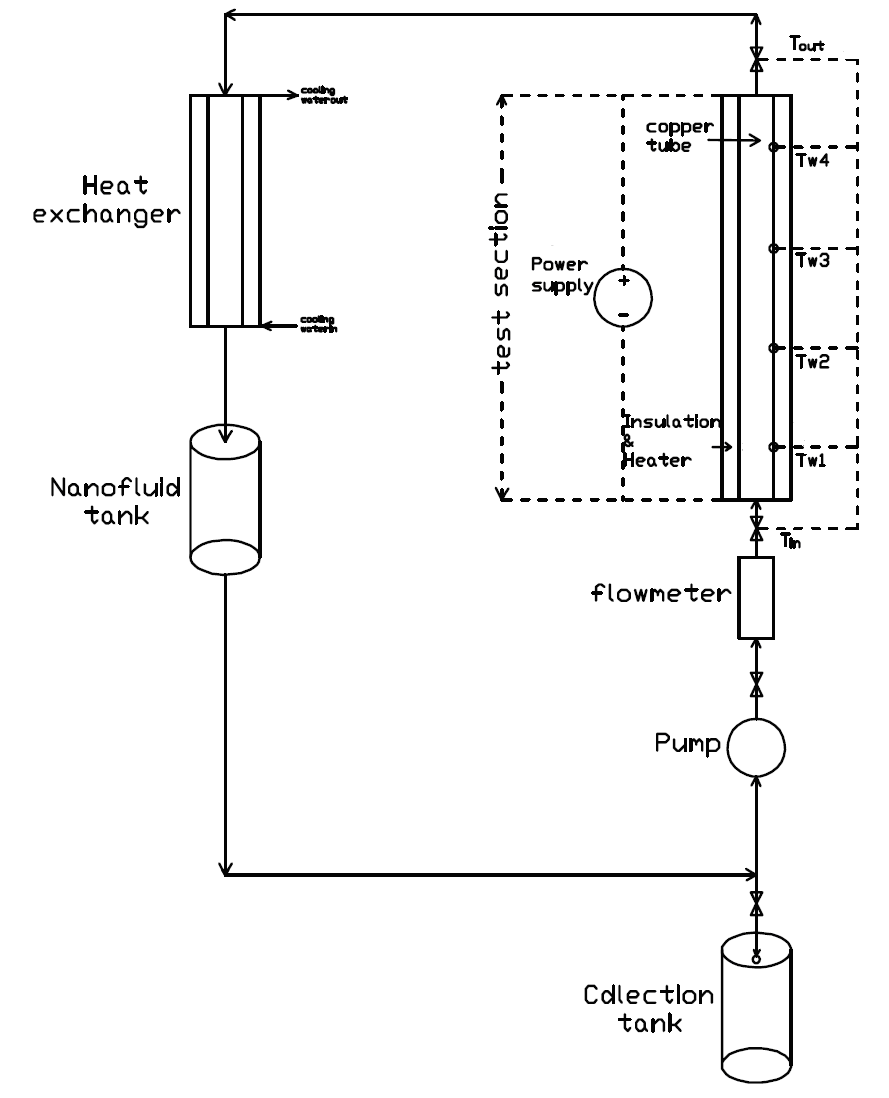
\includegraphics[width=0.9\linewidth]{fig1}
	\caption{}
	\label{fig:fig1}
\end{figure}

\begin{figure}
	\centering
	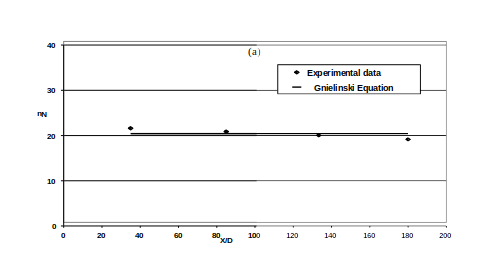
\includegraphics[width=0.8\linewidth]{fig2}
	\caption{}
	\label{fig:fig2}
\end{figure}

\begin{figure}
	\centering
	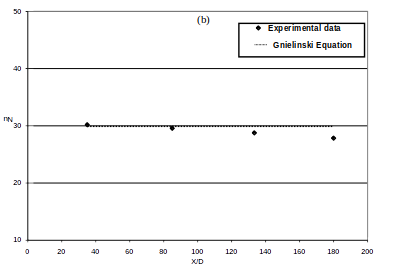
\includegraphics[width=0.8\linewidth]{fig3}
	\caption{}
	\label{fig:fig3}
\end{figure}

\begin{figure}
	\centering
	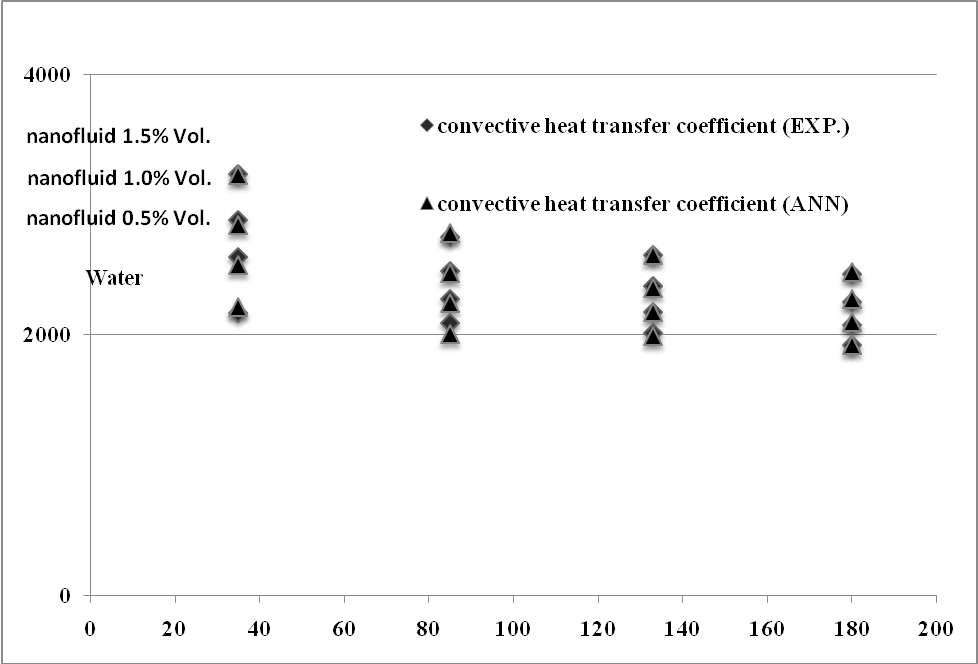
\includegraphics[width=0.9\linewidth]{fig4}
	\caption{}
	\label{fig:fig4}
\end{figure}

\begin{figure}
	\centering
	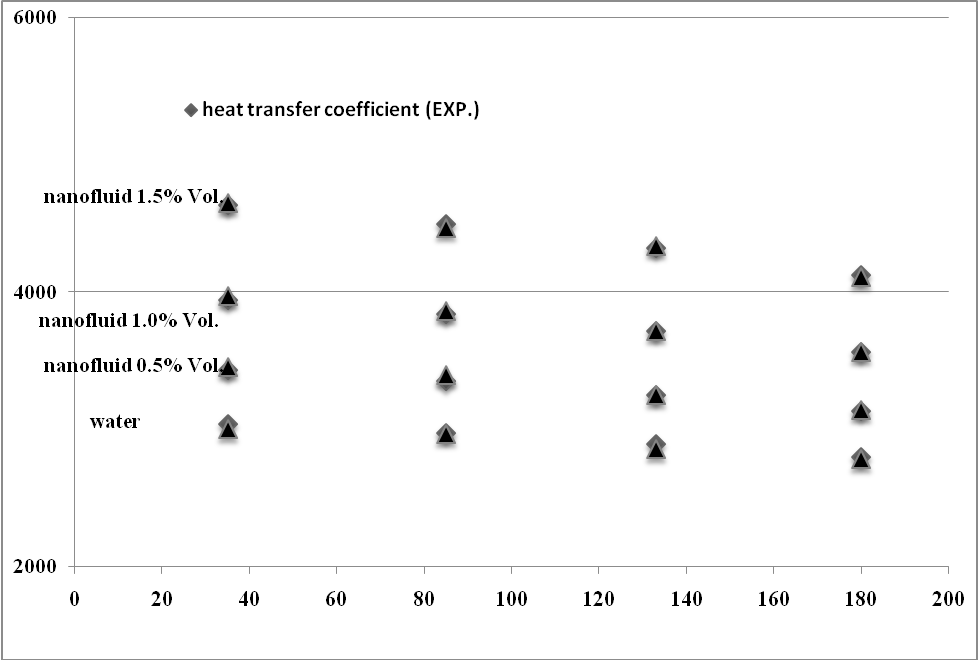
\includegraphics[width=0.7\linewidth]{fig5}
	\caption{}
	\label{fig:fig5}
\end{figure}

\begin{figure}
	\centering
	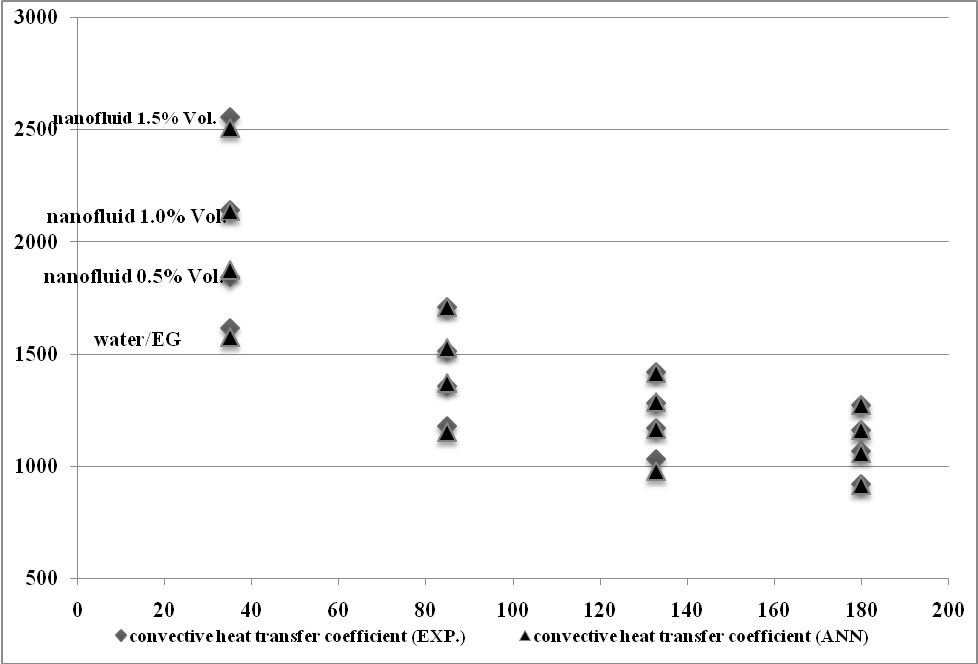
\includegraphics[width=0.8\linewidth]{fig8}
	\caption{}
	\label{fig:fig8}
\end{figure}


\begin{figure}
	\centering
	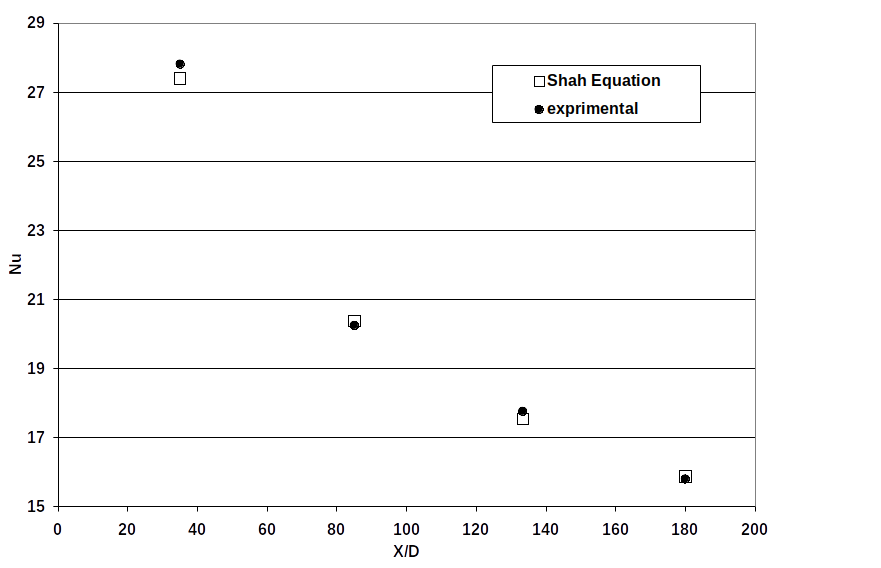
\includegraphics[width=0.9\linewidth]{fig6}
	\caption{}
	\label{fig:fig6}
\end{figure}


\begin{figure}
	\centering
	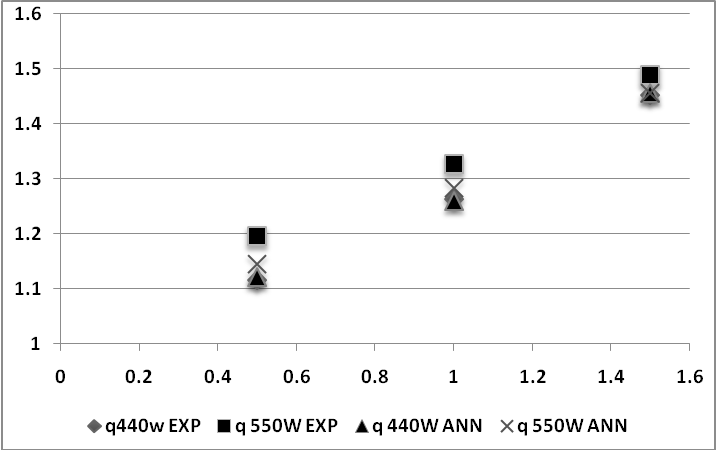
\includegraphics[width=0.7\linewidth]{fig9}
	\caption{}
	\label{fig:fig9}
\end{figure}


\begin{table}[htbp]
	\centering
	\caption{Comparison of various back propagation learning algorithms}
	\begin{tabular}{cccc}
		\hline
		R2 & MSE & Function & Back Propagation Algorithm \\
		\hline
		0.9899 & 0.0099 & trainrp & Resilient backpropagation (Rprop) \\
		0.9969 & 0.0031 & traincgf & Fletcher?Reeves conjugate gradient backpropagation \\
		0.9957 & 0.0042 & traincgp & Polak?Ribiere conjugate gradient backpropagation \\
		0.9960 & 0.0039 & traincgb & Powell?Beale conjugate gradient backpropagation \\
		0.9990 & 0.0010 & trainlm & Levenberg?Marquardt backpropagation \\
		0.9944 & 0.0112 & trainscg & Scaled conjugate gradient backpropagation \\
		0.9963 & 0.0037 & trainbfg & BFGS quasi-Newton backpropagation \\
		0.9957 & 0.0042 & trainoss & One step secant backpropagation \\
		0.9910 & 0.0089 & traingd & Batch gradient descent \\
		0.7778 & 0.2186 & traingdx & Variable learning rate backpropagation \\
		0.8963 & 0.1061 & traingdm & Batch gradient descent with momentum \\
		\hline
	\end{tabular}
\end{table}


\begin{table}[htbp]
	\centering
	\caption{Number of neurons in hidden layer with related mean square errors.}
	\begin{tabular}{cc}
		\hline
		MSE $\times 10^2$ & Number of Neurons \\
		\hline
		1.69 & 2 \\
		0.31 & 3 \\
		0.23 & 4 \\
		0.17 & 5 \\
		0.08 & 6 \\
		0.20 & 7 \\
		0.11 & 8 \\
		0.15 & 9 \\
		\hline
	\end{tabular}
\end{table}



%%===========================================================================================%%
%% If you are submitting to one of the Nature Portfolio journals, using the eJP submission   %%
%% system, please include the references within the manuscript file itself. You may do this  %%
%% by copying the reference list from your .bbl file, paste it into the main manuscript .tex %%
%% file, and delete the associated \verb+\bibliography+ commands.                            %%
%%===========================================================================================%%

\bibliography{sn-bibliography}% common bib file
%% if required, the content of .bbl file can be included here once bbl is generated
%%\input sn-article.bbl


\end{document}
